\subsection{Itinerary Optimisation Algorithms}

The following will evaluate the performance of the PSO
and GA optimisers. The tests were carried out using
200 POIs all around Malta.

Figure ~\ref{GAOptimisation} and figure ~\ref{PSOoptimise} show the scores of a seven-day
itinerary for the GA and PSO, respectively. The
algorithms are optimising throughout several
iterations for the following constraints:

\begin{itemize}
    \item Activity Pace: 2
    \item Number of days: 7
    \item Travel interest Vector:  beach=9, clubbing=8, bars=3, nature=4, shopping=2, museums=3.
\end{itemize}

\begin{figure}[h]
\centering
        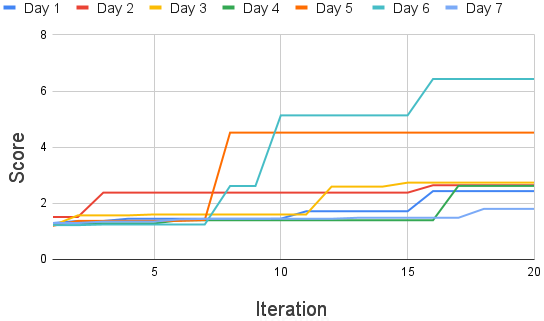
\includegraphics[width=0.65\textwidth]{GAOptimisation.png}
        \caption{GS 7-day optimisation.}
        \label{GAOptimisation}
\end{figure}

\begin{figure}[h]
\centering
        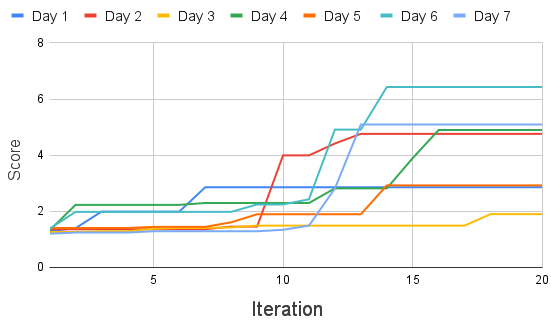
\includegraphics[width=0.65\textwidth]{PSOOptimisation.png} 
        \caption{PSO 7-day optimisation.}
        \label{PSOoptimise}
\end{figure}

%\begin{figure}[!htb]
    %\centering
    %\begin{minipage}{.58\textwidth}
        %%\centering
        %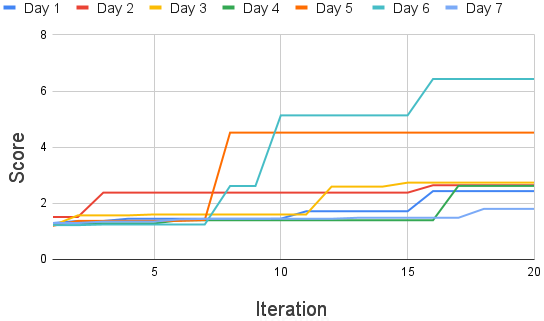
\includegraphics[width=0.85\textwidth]{GAOptimisation.png}
        %\caption{GS 7-day optimisation.}
        %\label{GAOptimisation}
    %\end{minipage}%
    %\begin{minipage}{0.58\textwidth}
        %%\centering
        %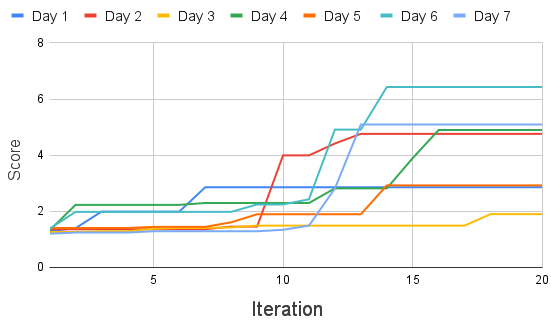
\includegraphics[width=0.85\textwidth]{PSOOptimisation.png} \caption{PSO 7-day optimisation.}
        %\label{PSOoptimise}
    %\end{minipage}

%\end{figure}


With 20 iterations and population size of 100, PSO
completed the optimisation in 15 seconds and achieved
an average score of 4.2. However, the GA completed the
task in 11 seconds and achieved an average score of
3.3.

Many parameters help tweak the performance of the
algorithms. In PSO, the inertia property heavily
controls the convergence behaviour (CITE). Out
algorithm implements the Time-Varying Inertia Weight
(CITE), which gradually decreases throughout each
iteration. Figure~\ref{Inertia} shows the optimisation algorithm
without the inertia property and barely increases the
score since the particles do not explore new
territories.

\begin{figure}[h]
\centering
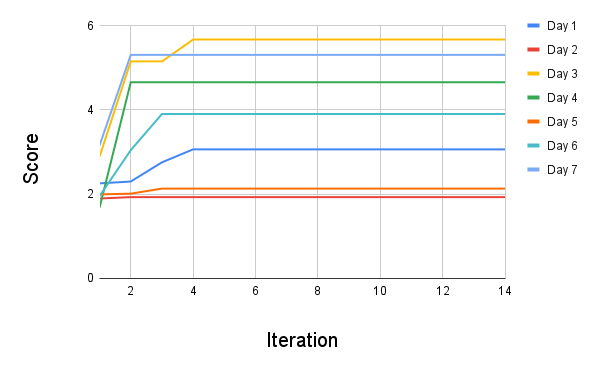
\includegraphics[width=0.6\textwidth]{Inertia.png}
\caption{PSO algorithm without intertia}
\label{Inertia}
\end{figure}

GAs are heavily affected by the crossover techniques
since the search for the best result is dependent on
the creation of new children (CITE). Figure X shows
the average scores of 20 generated itineraries for 
four different crossover techniques and the same
previously mentioned constraints. Since uniform
crossover achieved the highest average score, we will
be testing the rest of the results using this
technique.

\begin{figure}[h]
\centering
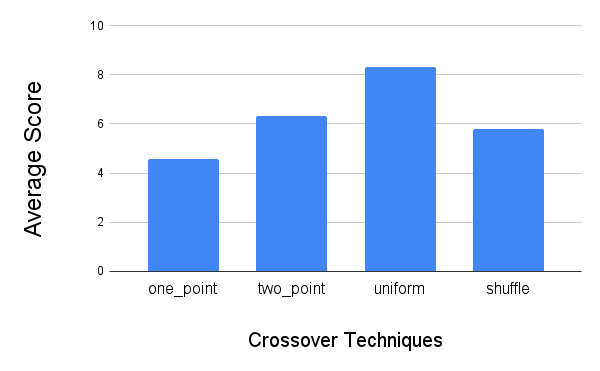
\includegraphics[width=0.6\textwidth]{Crossover.png}
\caption{Average Scores of different crossover techniques}
\label{RS}
\end{figure}


Table~\ref{Parameters} provides the parameter values of the two algorithms:

\begin{table}[h]

\centerline{
  \begin{tabular}{|l|c|c|} 
 \multicolumn{2}{c}{PSO}\\
 \hline
  \textbf{Parameter} & \textbf{Value} \\ 
 \hline
 Inetia & 7\\
 Personal acceleration& 2\\ 
 Global acceleration& 2\\ 
 Iterations& 20\\
 \hline
 \multicolumn{2}{c}{GA}\\
 \hline
 Iterations& 20\\
 Mutation probability& 0.2\\
 Parents portion& 0.3\\
 Elit ratio& 0.01\\
 Crossover technique& Uniform\\
 Crossover Probability& 0.5\\
 \hline
  \end{tabular}
}
\caption{All parameter values of the two algorithms} \label{t:tab}
\label{Parameters}
\end{table}

We generated 50 random constraints and tested them out
on both algorithms. Figure X shows how the number of
particles affects the score. For 100 population
members, both algorithms achieve similar average
scores. However, the difference in score is not
proportional to the average time taken to complete a
single day, as shown in figure X.

\begin{figure}[h]
\centering
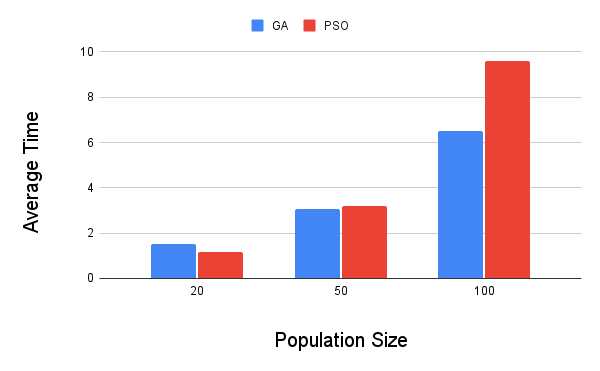
\includegraphics[width=0.6\textwidth]{AverageTime.png}
\caption{Average time spent for 50 iterations}
\label{AverageTime}
\end{figure}

\begin{figure}[h]
\centering
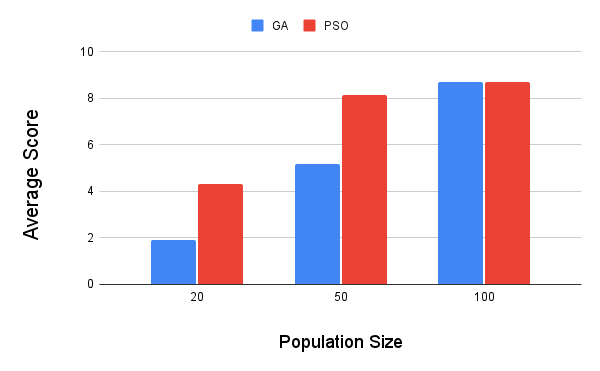
\includegraphics[width=0.6\textwidth]{AverageScore.png}
\caption{Average score achieved for 50 iterations}
\label{AverageScore}
\end{figure}


Through these results, we have shown how optimisation
meta-heuristics can provide a TTDP solution. However,
since other users will use the application, we didn't
want the generation's time to affect the user
experience. Since the difference between the average
score of 50 and 100 particles for PSO is only 0.5,
this variant provides the best balance of time and
score. Therefore it is the one chosen for our
application.   

